%!TEX root = ../master.tex
\chapter{Code Overview}\label{ch:codeover}

The structure of the implemented software can be seen in the class diagram in Figure~\ref{fig:implementedClassDiagram}.

\begin{figure}
	\centering
	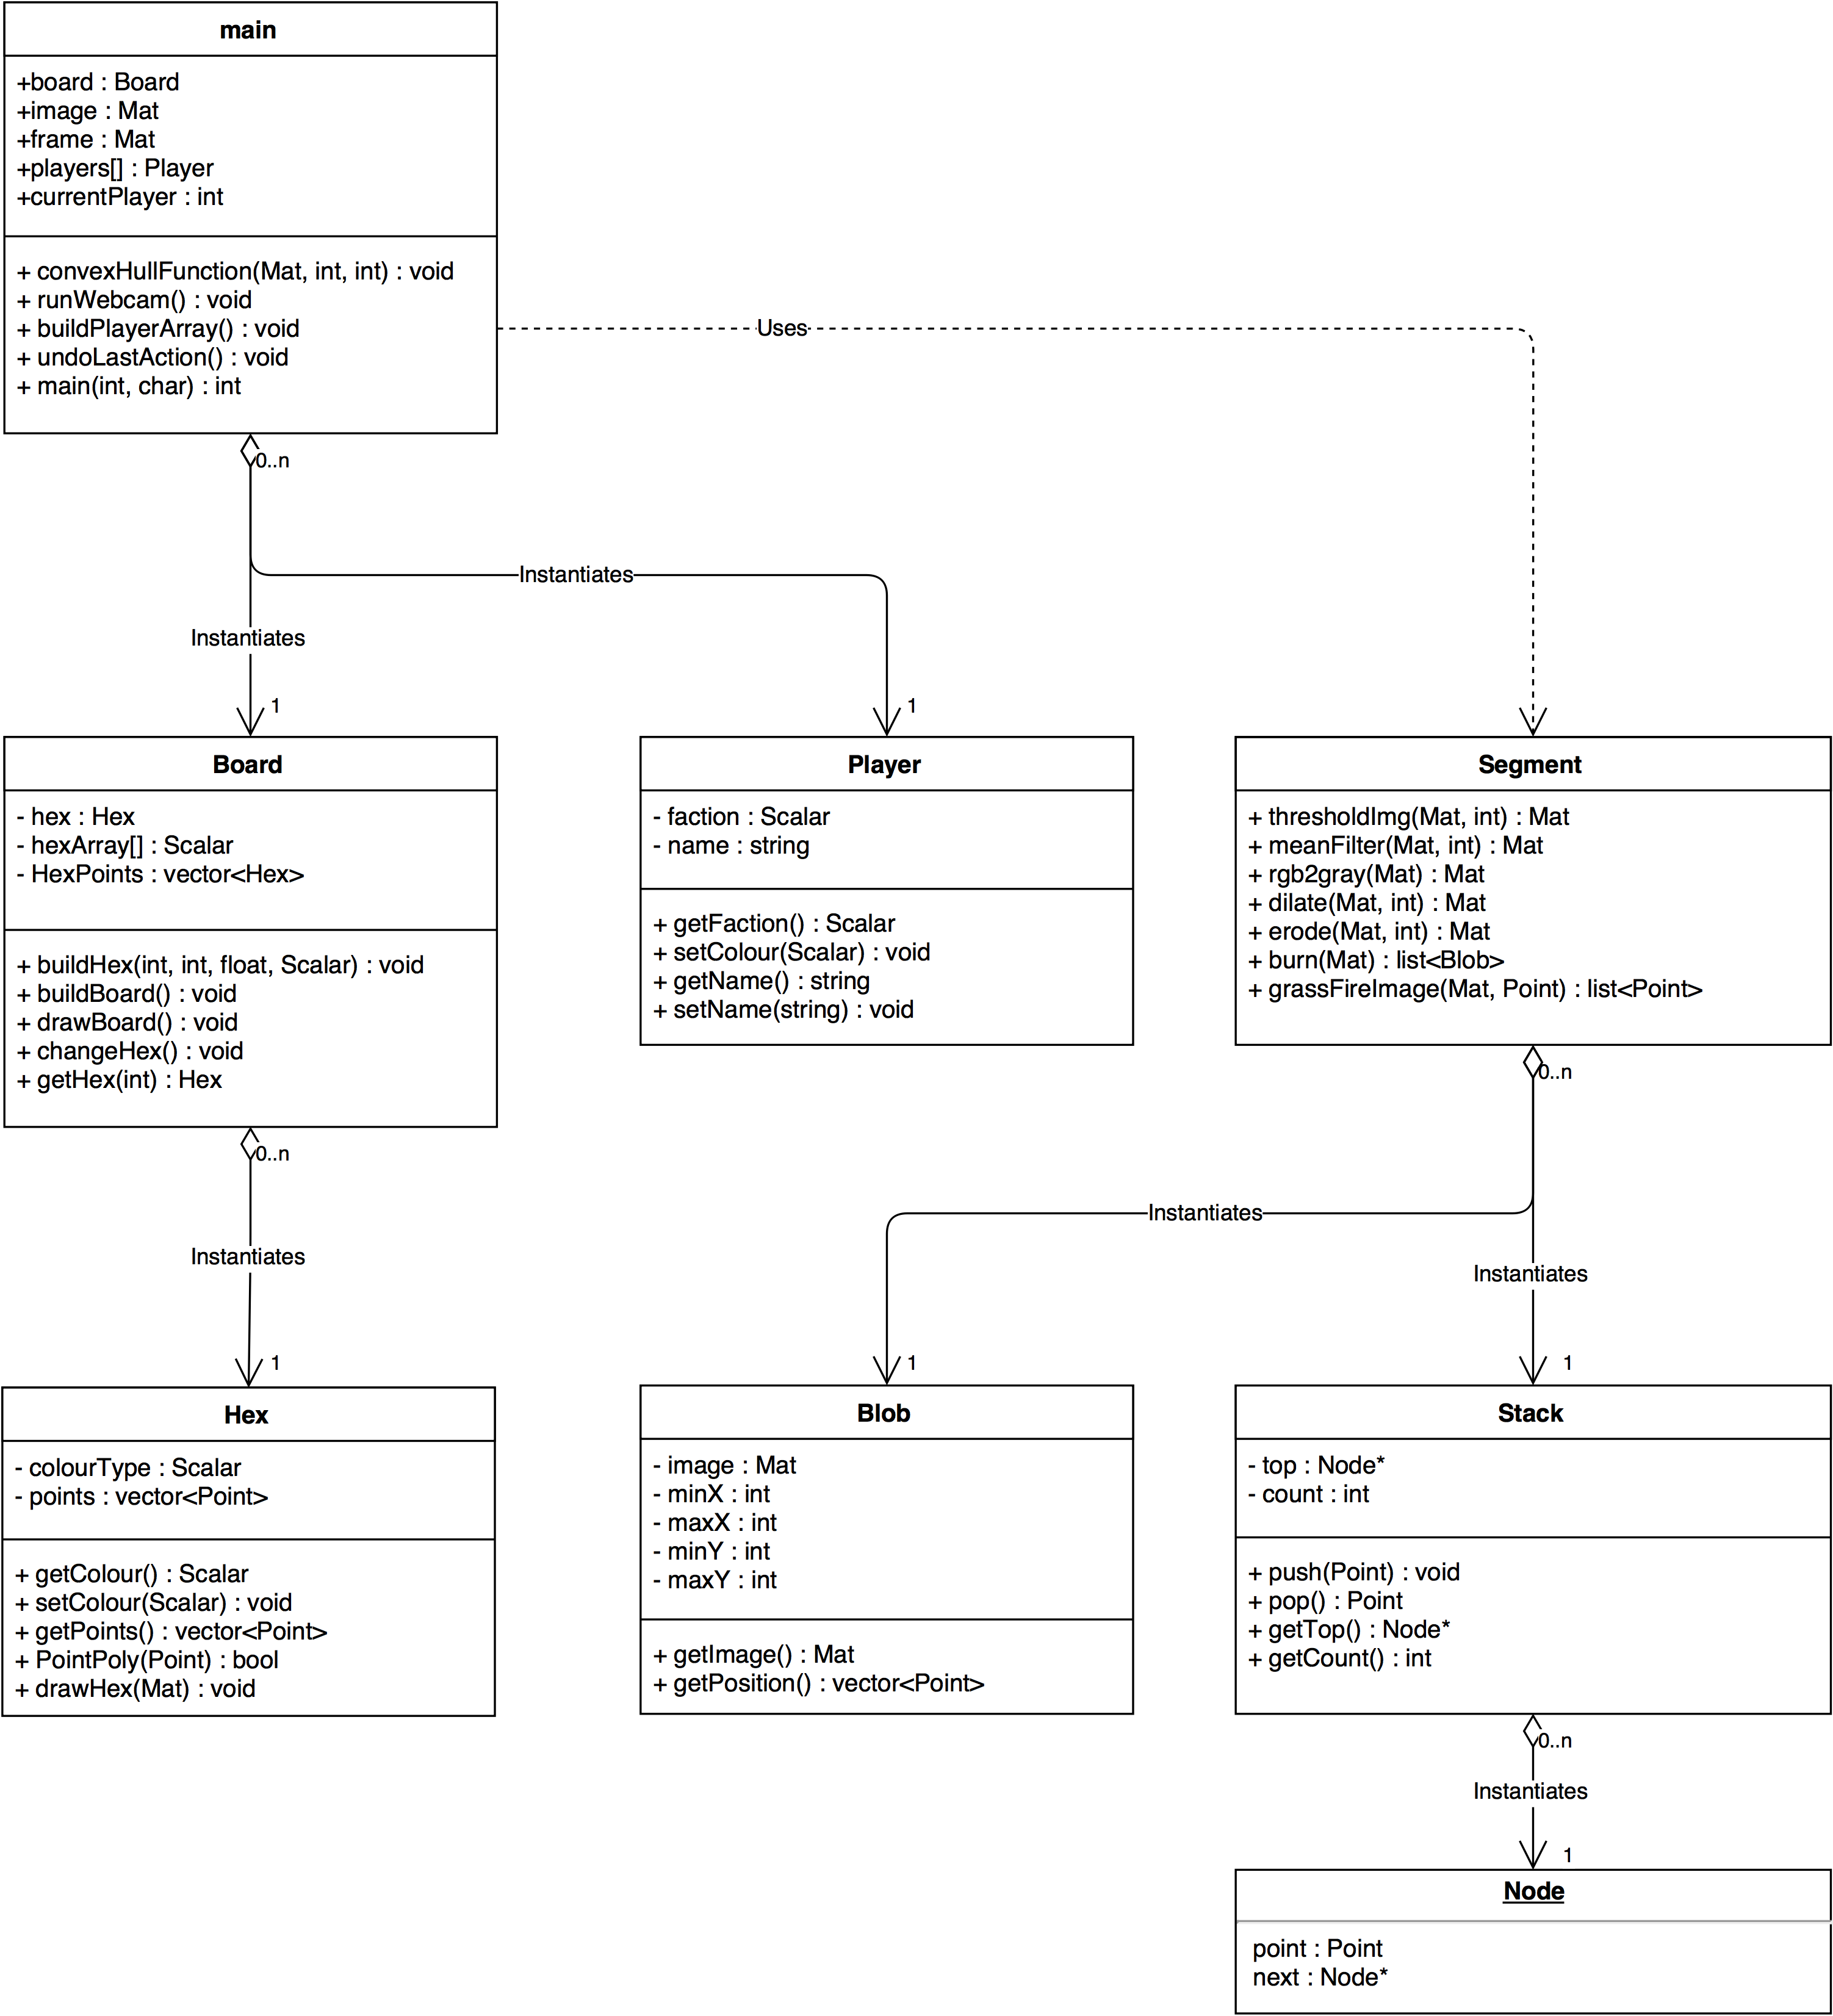
\includegraphics[width=1\textwidth]{ImplementedClassDiagram}
	\caption{Class diagram of the software \label{fig:implementedClassDiagram}}
	
\end{figure}


\section{Segment namespace}
\texttt{Segment} is a namespace which includes all image processing algorithms that have been implemented in this software. These methods are never called in the software due to poor CPU efficiency. They are included in this chapter to explain the principles of the used image processing method, and could easily be used in the main software instead of the OpenCV methods, if CPU power was not limited.

\subsection{Point-processing}
There are three point-processing algorithms in this software; an RGB-to-Greyscale colour conversion algorithm, a normalization algorithm, and a thresholding algorithm. All of these make use of double-nested \texttt{for}-loops to apply their operations to each pixel as shown in Figure~\ref{fig:pointprocess}.
\begin{figure}[!h]
\begin{lstlisting}
for (int y = 0; y < src.rows; ++y)
{
	for (int x = 0; x < src.cols; ++x)
	{
		//Code here...
	}
}
\end{lstlisting}
\caption{Basic point-processing algorithm. \label{fig:pointprocess}}
\end{figure} 

The RGB-to-Greyscale algorithm creates an 8-bit single-channel image and then maps the mean of the RGB-values of the input image pixels to the output like shown in Figure~\ref{fig:rgb2gray}

\begin{figure}[!h]
\begin{lstlisting}
output.at<uchar>(y, x) = (src.at<Vec3b>(y, x)[0] + src.at<Vec3b>(y, x)[1] + src.at<Vec3b>(y, x)[2]) / 3;
\end{lstlisting}
\caption{RGB-to-Greyscale operation.\label{fig:rgb2gray}}
\end{figure}

The normalization algorithm finds the maximum and minimum pixel values of the input image using an OpenCV function. It then processes each pixel to normalize them to a new maximum and minimum using the operation shown in Figure~\ref{fig:normalize}.

\begin{figure}
\begin{lstlisting}
output.at<uchar>(y, x) = floor((src.at<uchar>(y, x) - min) * (newMax - newMin) / (max - min) + newMin);
\end{lstlisting}
\caption{Normalization of a pixel. \label{fig:normalize}}
\end{figure} 

Finally, the thresholding algorithm determines whether a given output pixel is white or black based on the if-else statement that is shown in Figure~\ref{fig:threshold}.

\begin{figure}
\begin{lstlisting}
if (src.at<uchar>(y, x) >= threshold)
{
	src.at<uchar>(y, x) = 255;
}
else
{
	src.at<uchar>(y, x) = 0;
}
\end{lstlisting}
\caption{Thresholding. If the pixel value is above the threshold, make it white. Else, make it black.\label{fig:threshold}}
\end{figure}

\subsection{Neighbourhood processing}
The neighbourhood processing methods used in this software are \texttt{erode} and \texttt{dilate} These filters apply their kernels to each pixel through the process of convolution. That is to say, for each pixel they calculate a value for each pixel relative to the processed pixel based on the kernel. These results are then used for further calculations depending on the purpose of the filter.

The filters make use of a nested \texttt{for}-loop similar to the point-processing algorithms to go through each pixel. This loop can be seen in Figure~\ref{fig:neighbourhoodForLoop}. The main difference in this loop from the point-processing loop is, that this one ignores pixels at the edge of the image. This is to avoid \textit{out of bound} errors, since reading a pixel value outside an image causes OpenCV to throw an exception.

\begin{figure}
\begin{lstlisting}
for (int y = 0 + kernRad; y < src.rows - kernRad; ++y)
{
	for (int x = 0 + kernRad; x < src.cols - kernRad; ++x)
	{
		//Code here...
	}
}
\end{lstlisting}
\caption{Neighbourhood processing loop that reads each pixel in an image except those at the edge. \label{fig:neighbourhoodForLoop}}
\end{figure}

\texttt{erode} and \texttt{dilate} are essentially inversions of each other. They take binary images as arguments. \texttt{dilate} is what is known as a \texttt{hit} algorithm. It checks whether any pixel within the kernel is white (has a value of 255). If that is the case, the processed pixel is made white, otherwise it is made black. This can be seen in Figure~\ref{fig:dilateAlgorith}. \texttt{erode}, by contrast is a \textit{fit} algorithm. Like \texttt{dilate} it checks whether any pixel within the kernel is white. If any of the pixels in the kernel are not white, the pixel is made black. Only if all of the pixels are white will the processed pixel be white. This can be seen in Figure~\ref{fig:erodeAlgorithm}.

\begin{figure}
\begin{lstlisting}
for (int ky = y - kernRad; ky <= y + kernRad; ++ky)
{
	for (int kx = x - kernRad; kx <= x + kernRad; ++kx)
	{
		if (src.at<uchar>(ky, kx) == 255) {
			Temp++;
		}
	}
}
//if one of the pixels are value 255, give the output pixel greyscale value of 255
if (Temp != 0){
	output.at<uchar>(y, x) = 255;
}
//else, give it 0
else {
	output.at<uchar>(y, x) = 0;
}
Temp = 0;
\end{lstlisting}
\caption{The dilation algorithm. \label{fig:dilateAlgorith}}
\end{figure}

\begin{figure}
\begin{lstlisting}
for (int ky = y - kernRad; ky <= y + kernRad; ++ky)
{
	for (int kx = x - kernRad; kx <= x + kernRad; ++kx)
	{
		if (src.at<uchar>(ky, kx) == 255) {
			Temp++;
		}
	}
}
//if all the pixels are value 255, give the output pixel greyscale value of 255
if (Temp == kernPixels){
	output.at<uchar>(y, x) = 255;
}
//else, give it 0
else {
	output.at<uchar>(y, x) = 0;
}
Temp = 0;
\end{lstlisting}
\caption{The erotion algorithm.\label{fig:erodeAlgorithm}}
\end{figure}

\subsection{BLOB extraction}
For BLOB-extraction, two methods are used; \texttt{burn} and \texttt{grassFireImage}. \texttt{burn} performs two tasks; it calls \texttt{grassFireImage} when it finds a white pixel, and it builds an image from the list of pixels that are returned as a result. To find white pixels, a \texttt{for}-loop such as the one shown in Figure~{fig:pointprocess} is used. When a white pixel is found, \texttt{grassFireImage} is called. This method implements a sequential grass-fire algorithm to create a list of pixels from which a BLOB can be built. The method makes use of a linked list stack to keep track of the pixels that are currently being processed. As soon as a pixel is added to the stack, the pixel value is set to a non-white value to prevent pixels from being processed redundantly. This also ensures that \texttt{burn} does not call \texttt{grassFireImage} multiple times for the same blob. The algorithm is implemented for 4-neighbours connectivity. The code for this can be seen in Figure~\ref{fig:grassFireIf}. This code is contained within a \texttt{while}-loop, which runs for as long as elements are still present within the stack list. The nature of the if-else statements means that if any of the conditions are true, a new iteration of the loop will be started. If none of the pixels are white, the final block of code will be executed. Here the pixel is added to the \texttt{blopPoints} list and removed from the stack list. The next pixel in the stack list will then be processed. When the final pixel in the stack list has been removed, the \texttt{blobPoints} list is returned to the \texttt{burn} function, which contains the algorithm that builds an image from these points.

The dimensions of the BLOB image is determined by calculating the difference between the maximum and minimum x- and y-values in the returned list. Then the program iterates through the list to determine the position of each white pixel in the image. This image, as well as its maximum and minimum values are then added to a \texttt{Blob} object which is pushed to a list of BLOBs, that the rest of the software can use.  

\begin{figure}
\begin{lstlisting}
if (src.at<uchar>(point.y - 1, point.x) == 255) //if adjacent pixel is white 
{
	point = Point(point.x, point.y - 1);  //set adjacent pixel to be the current pixel
	src.at<uchar>(point.y, point.x) = 1;
	pointStack.push(point); //and put it into the stack
}
else if (
(...)
}
\end{lstlisting}
\caption{One of the if-statements in the grass-fire loop. This check is made for four of the pixel's neighbours. \label{fig:grassFireIf}}
\end{figure}

\section{Stack list}
The stack list implementation makes use of a singly linked of a \texttt{Node} struct which contains a point, and a memory pointer to the next entry in the list, as well as a counter which records the amount of entries in the list. This class has four public methods. \texttt{push} adds a new \texttt{Node} to the top of the list, \texttt{pop} destroys the top-most \texttt{Node} in the list and returns its data, \texttt{getTop} simply returns the top-most \texttt{Node}, and \texttt{getCount} returns the \texttt{count} value.


\section{Board class}
The \texttt{Board} class is responsible for determining the position of each hexagon on the board, handling the colour of each hexagon, and rendering the image. 

\begin{figure}
\begin{lstlisting}
for (int i = 0; i < 12; i++){
	x1 += 2 * h;
	buildHex(x1, y, h, hexArray[i]);
}
\end{lstlisting}
\caption{One of the \texttt{for}-loops used in the \texttt{buildHex} method. A loop has been implemented for each row on the board. \label{fig:buildHexForLoop}}
\end{figure}

The rendered board consists of a hexagonal grid placed on top of a pre-made image. Each hexagon is labeled from 0 to 111. Two methods are used to build these hexes. In the \texttt{buildBoard} method, the values defined in the \texttt{Colour} class are assigned to a Scalar array which are used to define the colour of each hexagon. A set of \texttt{for}-loops - one of which can be seen in Figure~\ref{fig:buildHexForLoop} - goes through each desired center position of the hexagons. For each of these positions, the \texttt{buildHex} method is called. The hexagons are built as instantiated \texttt{Hex} objects which take a list of six Points and a Scalar as arguments in their constructor. Finally, the method pushes the \texttt{Hex} object to a list. The code for this can be seen in Figure~\ref{fig:buildHexMethod}. Each Point in the \texttt{Hex} represents a corner in a hexagon which is drawn with the OpenCV \texttt{fillConvexPoly} method. This method is called in the \texttt{drawHex} method which is contained in the \texttt{Hex} class. After each hexagon has been built, the \texttt{drawBoard} method can be called continuously. This method simply calls the \texttt{drawHex} method for each \texttt{Hex}.

\begin{figure}
\begin{lstlisting}
float r = (2.0 / 3.0) * (sqrt(3.0) * h);

Point a(x, y);
Point b(x + h, y + (0.5*r));
Point c(x + h, y + (1.5*r));
Point d(x, y + (2 * r));
Point e(x - h, y + (1.5*r));
Point f(x - h, y + (0.5*r));
vector<Point> pointsVec = { a, b, c, d, e, f };

Hex hex = Hex(colour, pointsVec);
HexPoints.push_back(hex);
\end{lstlisting}
\caption{The contents of the \texttt{buildHex} method. \label{fig:buildHexMethod}}
\end{figure}

Finally the \texttt{Board} class contains a \texttt{changeHex} and \texttt{getHex} method. The former takes an \texttt{int} and a \texttt{Scalar} as arguments which are used to call the \texttt{setColour} method of a desired \texttt{Hex} in the list to set it to a desired colour. The latter method simply returns the \texttt{Hex} object at a desired position in the list of hexagons.

\section{Main function}
The main function is executed when the software is started. This function initially reads the board image from disk and loads it into a window. Then a \texttt{Board} object is instantiated and its \texttt{buildBoard} method is called. Then an array of \texttt{Player} objects is defined after which the main loop is started. In this loop, an image from the camera is received and processed with OpenCV methods. These methods convert the image to greyscale, apply a gaussian blur, and then segment the image using a simple, static threshold. An opening algorithm (erode, then dilate) is finally applied to the thresholded image.

\begin{figure}
\begin{lstlisting}
\end{lstlisting}
\end{figure}